\subsection{Contexto da pesquisa} \label{subsec:contexto}
\citeonline{mateus} A necessidade de desenvolvimento do planejamento estratégico no mundo corporativo e no dia-a-dia torna a análise de séries temporais e previsões valiosas ferramentas para apoiar o processo de tomada de decisão a curto, médio e longo prazo. Devido a não linearidades, sazonalidade, tendência e ciclicidade nos dados temporais, o desenvolvimento de modelos de previsão eficientes é uma tarefa desafiadora. 

No conjunto de dados da SANEPAR, há um volume significativo no consumo de água e, com as interrupções que a cidade tem enfrentado, é necessário analisar os dados para compreender melhor os padrões de interrupção no abastecimento e os picos de consumo ao longo das horas e dias.

Nesta dissertação, será realizada uma revisão sistemática de modelos preditivos para avaliar o melhor modelo que pode ser utilizado e como ele pode ser validado para prever a escassez de água. Essas análises serão feitas utilizando a linguagem de programação \textit{Python}.

A abordagem deste trabalho consiste em explorar o conceito de séries temporais e sua aplicação no campo do aprendizado de máquina. Os dados de séries temporais referem-se a dados coletados e armazenados ao longo do tempo, permitindo que observadores identifiquem anomalias nos dados. A classificação dos dados por ano ou dia é essencial na análise de séries temporais, e se os dados forem atribuídos aleatoriamente, pode ser mais desafiador fazer previsões e tomar decisões com base nos dados coletados.

É importante destacar que a análise de médias pode ser enganosa se não forem excluídos os valores discrepantes, também conhecidos como ``\textit{outliers}''. Esses valores discrepantes podem levar a resultados extremamente altos ou baixos que não refletem a realidade.

O campo do aprendizado de máquina abrange várias áreas, conforme ilustrado na Figura \ref{fig:paradigma-ml}. Serão explorados os diferentes componentes do aprendizado de máquina e como eles podem ser aplicados em diversos contextos.
 
\begin{figure}[H]
	\centering
	\caption{Paradigma de aprendizado de máquina}
	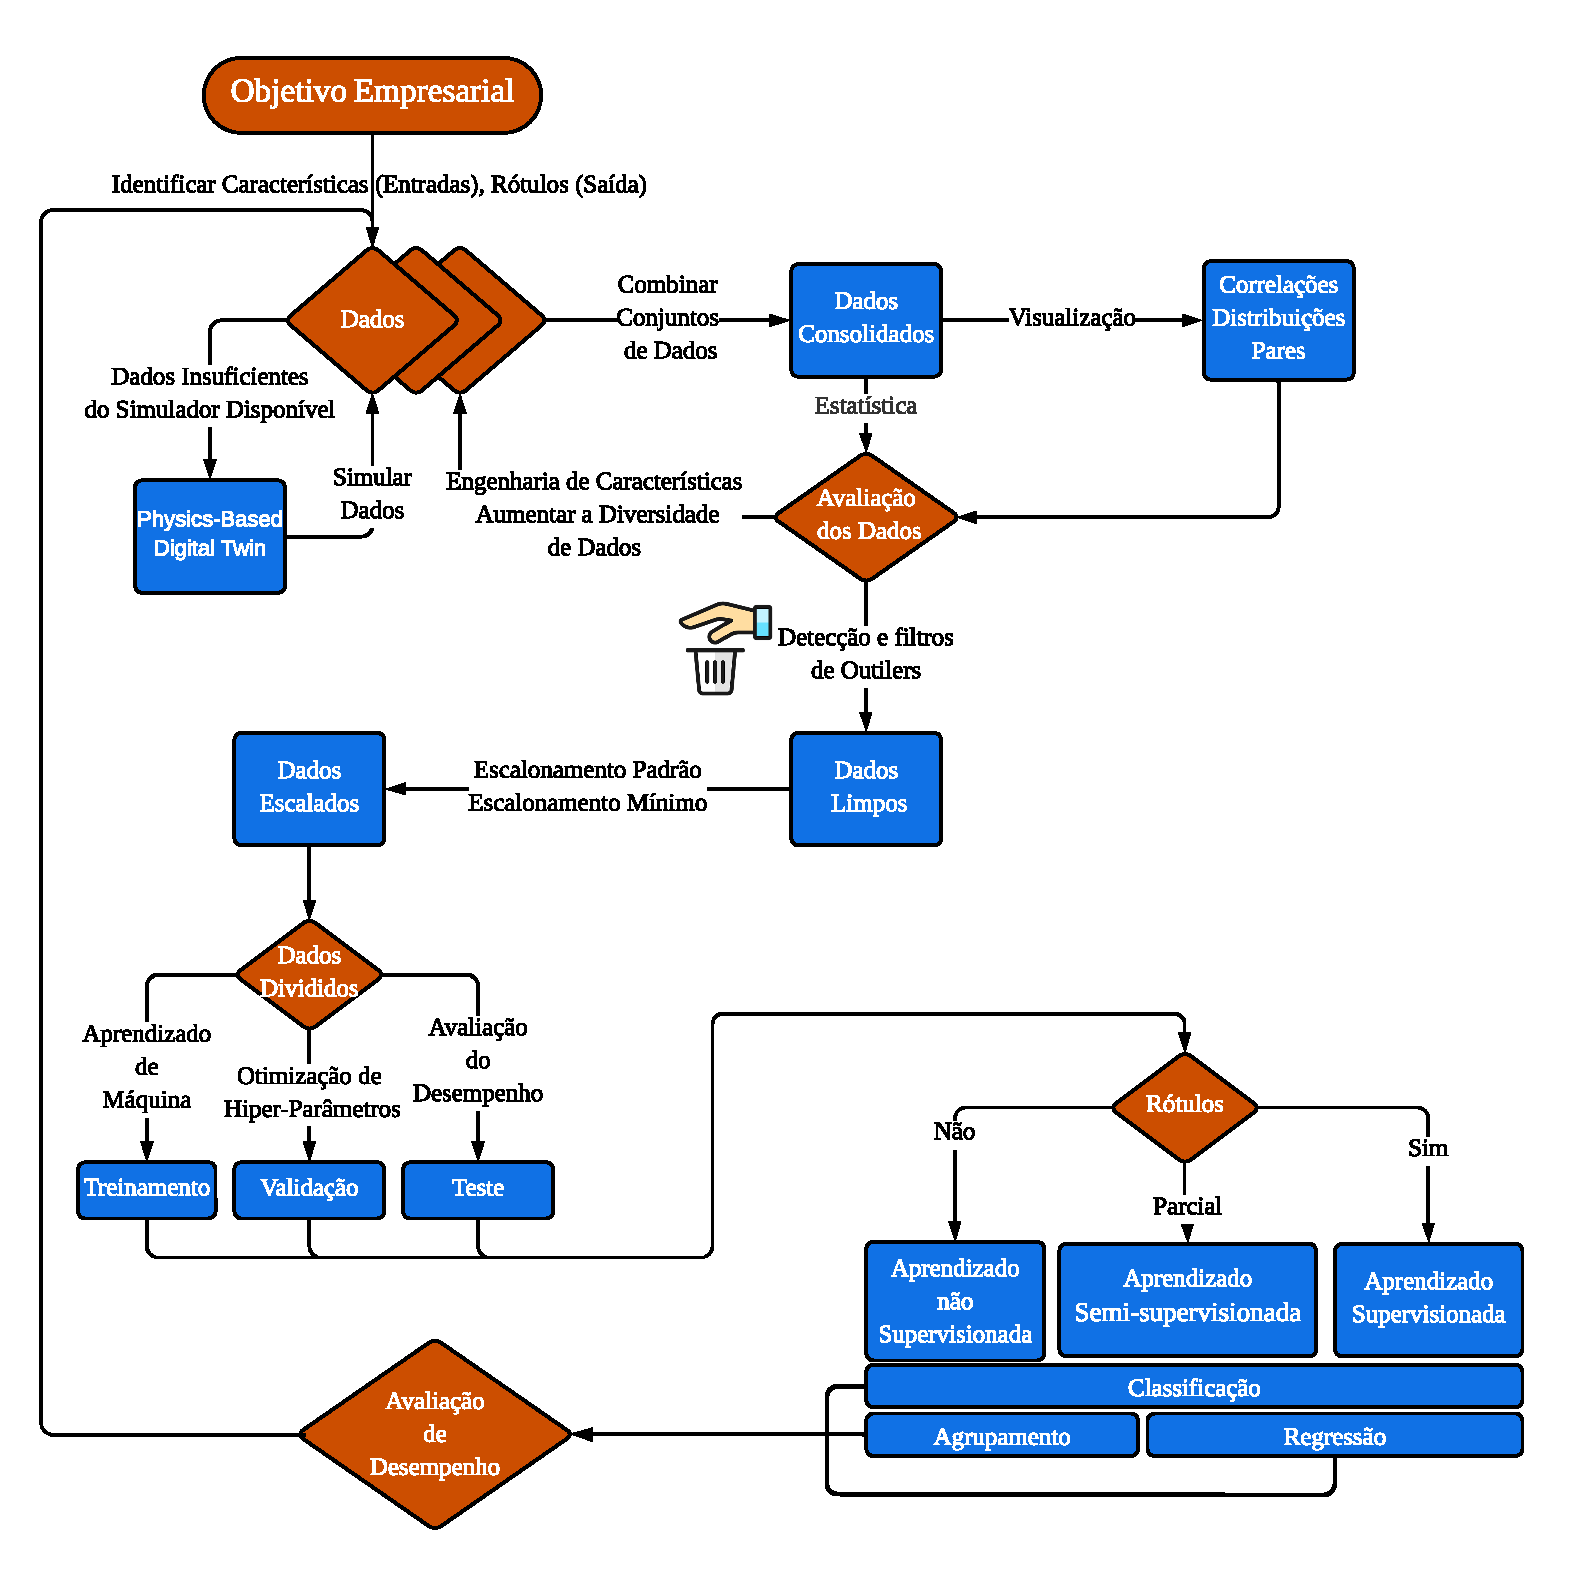
\includegraphics[width=1\linewidth]{Introducao/Figuras/paradigma-ml}
	
	Fonte: Elaboração própria
	\label{fig:paradigma-ml}
\end{figure}
  
      
\subsubsection{Motiva\c c\~ao da pesquisa} \label{subsubsec:motivacao}
   %Escrever algo motivador 
    
    De acordo com \cite{vasconcelos_2020} Curitiba e região metropolitana enfrentou um rodízio com $36$ horas com água e $36$ horas sem abastecimento. A média geral dos reservatórios da região está em $27,96\%$ da capacidade. Assim em medida a isso essa pesquisa tem como a abordagem da falta de água, essa falta que pode ser vista como uma seca, em média nos anos anteriores de 2020 a chuva tem marcado a quantia de $1.704$ mm. \cite{vasconcelos_2020} Desde 2016, quando registrou 1.704 mm de chuva, Curitiba não atingiu mais a média anual de precipitação, que é de 1.490 mm, com base em dados da estação pluviométrica do IBMET.  Apesar de abaixo da média, o mínimo registrado desde então ocorreu em 2020, com 1.158 mm.
    
   Em meio a essa motivação, é possível realizar uma análise mais aprofundada dos dados fornecidos pela SANEPAR, a fim de prever e evitar a ocorrência de escassez de água, que foi registrada juntamente com a anomalia detectada em 2020. Com o retorno das chuvas, houve um aumento no nível dos reservatórios.
    
    